\documentclass[11pt]{article}
\usepackage[margin=1in]{geometry}
\usepackage{amsmath,amssymb}
\usepackage{graphicx}
\usepackage{booktabs}
\usepackage[hidelinks]{hyperref}
\usepackage{enumitem}
\setlist{itemsep=2pt,topsep=4pt}
\graphicspath{{weekly_note_figs/}}
\newcommand{\dd}{\mathrm{d}}
\newcommand{\tr}{\operatorname{tr}}
%%NUMBERS%%

\title{Weekly note, 22 November 2026\\[2pt]\large Wave computing: research design, the math, and a first wave simulation}
\author{William Starks}
\date{}

\begin{document}
\maketitle

\section*{Summary}
\begin{itemize}
\item \textbf{Research design.} A camera records only brightness, but the grain of a laser spot (speckle) is
  interference, and its statistics are squared correlations of the light field. So the wave information is in the
  frames we can already take. Section~\ref{sec:design} states what we measure, what it says about the material, and how
  each claim is checked.
\item \textbf{Math.} Section~\ref{sec:math} derives one formula for the speckle contrast of a frame (F1) and two for the
  speckle correlation between frames, when the wavelength is stepped (F3) and when the beam is moved (F4). Each is the
  Fourier transform of something the material decides: how far light travels inside it, and how far sideways.
\item \textbf{Simulation, three levels.} (1) The wave equation solved exactly for \fwN{} scatterers. (2) A Monte Carlo
  that follows light paths with their length and polarization. (3) Camera frames with speckle, noise and pixels,
  generated from (2). No real data is used; the materials are made-up parameter sets.
\item \textbf{Result.} The exact wave solution agrees with the path formulas within \fwSpecDiff{} (wavelength steps) and
  \fwTiltDiff{} (beam tilts) in correlation, with nothing fitted. The simulated frames follow F1 within
  \mWorstMulti\% in every ring, and F3 and F4 within \wlRms{} in correlation on average (\beamWorst{} at worst).
  Of the seven predictions written down beforehand, three held in full and four were missed in part, each narrowly;
  all are reported in Section~\ref{sec:results}.
\item \textbf{Two things I got wrong, now corrected.} The ``move the beam a fraction of a millimetre'' test does not
  work with a collimated beam; it needs a diverging beam or steps as large as the beam (Section~\ref{sec:beam}). And
  light keeps its polarization a little farther than I predicted (\polDist{} mean free paths, not 5).
\item \textbf{For the rig.} Zooming in is right: the spot has to cover many speckle grains. A cheap multimode laser
  diode is better than a single-frequency laser for the ring-by-ring speckle method. Section~\ref{sec:rig} has the
  numbers.
\end{itemize}

\section{Research design}\label{sec:design}

\paragraph{Question.} Can a few lasers and a camera name the material of an object from the physics of how its
surface and bulk return light, in a way that does not depend on the object's colour, print, brightness or shape?

\paragraph{Idea.} Light that comes back from a laser spot took many paths. Some were reflected at the surface. Some
went into the material, were scattered many times, and came out a little to the side. The camera adds the fields of
all these paths. Three properties of the paths depend on the material and not on how the object looks:
\begin{enumerate}
\item how long the paths inside the material are (their spread sets how fast speckle changes with wavelength, and how
  much of it survives a laser with a short coherence length);
\item how far sideways the light travels (it sets how fast speckle changes when the beam is tilted or moved, and the
  size of the glow around the spot);
\item whether the light keeps its polarization (surface light does, light from inside does not).
\end{enumerate}
Brightness and colour change the amount of light, not these three. Each method below reads one of them from
normalized quantities (contrast and correlation), which do not change when the light is dimmer or a different colour.

\paragraph{Methods.} Numbering as in my message of 20 November.
\begin{description}[leftmargin=1.2em,itemsep=2pt]
\item[1. Speckle.] The number of independent speckle patterns $M$ in a frame, ring by ring outward from the spot
  centre (formula F1). $M=1$ for surface light; it rises where light has travelled inside.
\item[2. Scattering fit.] The mean brightness profile of the spot, fitted as surface light plus light from inside,
  with lengths measured in beam widths. This uses the same transport kernel $K$ as below, without the speckle.
\item[4. Wave computing.] The object itself is the reservoir: a fixed random medium that transforms the light we send
  in. We control the inputs (wavelength, beam position or tilt, which laser), the camera reads the outputs, and only a
  linear readout is trained. The readout is trained on the correlations between the outputs for different inputs (F3,
  F4), because those depend on the material's statistics and not on the particular object.
\item[3. Polarization] waits for the device. With polarizers, F1 splits into its two parts: loss of polarization and
  spread of path length.
\end{description}

\paragraph{How each claim is checked.} Before accuracy counts, a feature must (a) agree between the scanner's two red
lasers, (b) agree between two poses of the same object, (c) not follow the object's visible brightness and colour
within a material, and (d) name the material of objects that were never in training. Plans are written in the lab
notebook before scoring (repository \texttt{greatroboticslab/wavecomputing}, \texttt{EXPERIMENT\_LOG.md}).

\paragraph{Where we are.} On the scanner previews we have (800-pixel JPEGs, spot cores overexposed) the features
failed checks (a) to (d); those files cannot test the methods (notebook entry (n)). This week replaces the missing
data with theory and simulation: is the math right, and what must the camera and laser do for the methods to work?
Real captures come next (Section~\ref{sec:next}).

\section{The math}\label{sec:math}

\paragraph{What reaches a pixel.} Let the laser have wavenumber $k=2\pi/\lambda$. Path $p$ leaves the surface at
$\mathbf{x}_p$ after a length $s_p$ inside the material (refractive index $n$), with amplitude $\mathbf{a}_p$ (a
2-vector, its polarization). The field leaving the surface and the field in the image are
\begin{equation}
\mathbf{E}(\mathbf{x};k)=\sum_p \mathbf{a}_p\,e^{\,i k n s_p}\,\delta(\mathbf{x}-\mathbf{x}_p),\qquad
\mathbf{U}(\mathbf{x};k)=\int h(\mathbf{x}-\mathbf{x}')\,\mathbf{E}(\mathbf{x}';k)\,\dd^2x' ,
\end{equation}
where $h$ is the lens's amplitude point-spread function (set by its aperture). Light reflected at the surface is the
term $s_p=0$. The camera records
\begin{equation}
I(\mathbf{x})=\int S(k)\,\bigl|\mathbf{U}(\mathbf{x};k)\bigr|^2\,\dd k ,
\end{equation}
summed over the two polarizations and over the laser's spectrum $S(k)$ (normalized to 1), because different
polarizations and different laser lines do not interfere on the sensor.

\paragraph{Why brightness is enough.} A resolution cell of the lens collects very many paths with unrelated phases,
so $\mathbf{U}$ is a complex Gaussian random field. A Gaussian field is fully described by its covariance
\begin{equation}
\Gamma(\mathbf{x};k,k')=\bigl\langle \mathbf{U}(\mathbf{x};k)\,\mathbf{U}^\dagger(\mathbf{x};k')\bigr\rangle
=\int W(\mathbf{x},s)\,e^{\,i(k-k')ns}\,\dd s ,
\label{eq:gamma}
\end{equation}
where $W(\mathbf{x},s)$ is the $2\times2$ polarization coherency matrix of the light that leaves near $\mathbf{x}$
after path length $s$ (cross terms between different paths average to zero). For Gaussian fields the covariance of
two intensities is the squared modulus of the covariance of the two fields:
\begin{equation}
\langle I_a I_b\rangle-\langle I_a\rangle\langle I_b\rangle=\bigl\|\langle \mathbf{U}_a\mathbf{U}_b^\dagger\rangle\bigr\|_F^2 .
\label{eq:siegert}
\end{equation}
This is the point of the whole approach. We do not record the wave, but the variance of speckle and the correlation
between two speckle frames \emph{are} field correlations, squared. Everything below follows from
\eqref{eq:gamma} and \eqref{eq:siegert}.

\paragraph{F1: speckle contrast of one frame.} With $\gamma(\Delta)=\int S(k)e^{ik\Delta}\dd k$ the laser's degree of
temporal coherence at optical path difference $\Delta$, the contrast $K=\sigma_I/\langle I\rangle$ at $\mathbf{x}$ is
\begin{equation}
K^2(\mathbf{x})=\frac{\displaystyle\iint \tr\!\bigl[W(\mathbf{x},s)\,W(\mathbf{x},s')\bigr]\,
\bigl|\gamma\bigl(n(s-s')\bigr)\bigr|^2\,\dd s\,\dd s'}{\Bigl(\displaystyle\int \tr W(\mathbf{x},s)\,\dd s\Bigr)^2},
\qquad M=\frac{1}{K^2}. \tag{F1}
\end{equation}
$M$ counts the independent speckle patterns that add up in the frame. Three limits make it concrete:
\begin{itemize}
\item Single-frequency laser ($\gamma\equiv1$): $K^2=(1+P^2)/2$, with $P$ the degree of polarization of the returned
  light. Surface light ($P=1$) gives $M=1$; fully depolarized light gives $M=2$, and no more.
\item A share $f$ of surface light on top of depolarized light from inside, single-frequency laser: $K^2=(1+f^2)/2$.
\item A laser whose coherence length $L_c$ is shorter than the spread $\Delta s$ of optical path lengths: paths that
  differ by more than $L_c$ no longer interfere, and $M$ grows roughly as $2\,\Delta s/L_c$. This is how $M$ reads path
  length.
\end{itemize}

\paragraph{F2: path lengths from diffusion.} Far from the entry point light diffuses. Let
$R(\rho;\mu_a)$ be the light leaving at distance $\rho$ from a pencil beam for absorption $\mu_a$ (the standard
dipole formula, below). A path of length $s$ carries the weight $e^{-\mu_a s}$ and the phase $e^{\,i\,n\,\Delta k\,s}$,
so the Fourier transform over path length is the same formula with a complex absorption:
\begin{equation}
\frac{\displaystyle\int p(s\,|\,\rho)\,e^{\,i\,n\,\Delta k\,s}\,\dd s}{\displaystyle\int p(s\,|\,\rho)\,\dd s}
=\frac{R(\rho;\ \mu_a-i\,n\,\Delta k)}{R(\rho;\ \mu_a)} . \tag{F2}
\end{equation}
With transport length $\ell^*$, $D=\ell^*/3$, $\kappa=\sqrt{\mu/D}$, $z_0=\ell^*$, $z_b=2AD$ ($A=1$ for a matched
surface), $r_1^2=z_0^2+\rho^2$ and $r_2^2=(z_0+2z_b)^2+\rho^2$,
\begin{equation}
R(\rho;\mu)=\frac{1}{4\pi}\Bigl[\frac{1}{4\pi D}\Bigl(\frac{e^{-\kappa r_1}}{r_1}-\frac{e^{-\kappa r_2}}{r_2}\Bigr)
+\frac{3}{4\pi}\Bigl(z_0\bigl(\kappa+\tfrac{1}{r_1}\bigr)\frac{e^{-\kappa r_1}}{r_1^2}
+(z_0+2z_b)\bigl(\kappa+\tfrac{1}{r_2}\bigr)\frac{e^{-\kappa r_2}}{r_2^2}\Bigr)\Bigr].
\end{equation}
For a real beam, $R$ is convolved with the beam profile.

\paragraph{F3: stepping the wavelength.} Two frames taken with a single-frequency laser at wavenumbers $\Delta k$
apart have the speckle correlation
\begin{equation}
C(\Delta k)=\frac{\|\Gamma(\Delta k)\|_F^2}{\|\Gamma(0)\|_F^2},\qquad
\Gamma(\Delta k)=\int W(\mathbf{x},s)\,e^{\,i\,\Delta k\,n\,s}\,\dd s . \tag{F3}
\end{equation}
The speckle computes the squared Fourier transform of the path-length distribution. Surface light has $s=0$ and
never decorrelates, so the curve levels off at a plateau set by the surface share; light from inside decorrelates at
a step $\Delta\lambda\approx\lambda^2/(2\pi n\,\Delta s)$, which is 0.05~nm for a 1~mm spread at 635~nm.

\paragraph{F4: moving the beam.}\label{par:f4} Let $A(\mathbf{x})$ be the beam's field on the object and
$K(\mathbf{x}-\mathbf{x}')$ the transport kernel (light leaving at $\mathbf{x}$ per unit light entering at
$\mathbf{x}'$). The light at image point $\mathbf{x}$ is fed from entry points distributed as
$F_{\mathbf{x}}(\mathbf{x}')=(|h|^2*K)(\mathbf{x}-\mathbf{x}')$. With the beam at $\mathbf{a}$ and then at
$\mathbf{b}$, the two fields at $\mathbf{x}$ have the covariance
\begin{equation}
\Gamma_{ab}(\mathbf{x})=\int F_{\mathbf{x}}(\mathbf{x}')\,A(\mathbf{x}'-\mathbf{a})\,A^*(\mathbf{x}'-\mathbf{b})\,\dd^2x',
\qquad C_{ab}=\frac{|\Gamma_{ab}|^2}{\Gamma_{aa}\,\Gamma_{bb}} \tag{F4}
\end{equation}
(per polarization). Two cases:
\begin{itemize}
\item \emph{Flat wavefront} (collimated beam, $1/e^2$ radius $w$, step $d$): $A(\mathbf{x}'-\mathbf{a})A^*(\mathbf{x}'-\mathbf{b})$
  is real and smooth, and
  \begin{equation}
  C=e^{-d^2/w^2}\;\frac{H(\mathbf{x}-\mathbf{d}/2)^2}{H(\mathbf{x})\,H(\mathbf{x}-\mathbf{d})},
  \end{equation}
  with $H$ the mean brightness of the spot. The last factor is 1 or more inside the spot and within a few per cent of
  1 in the glow. A step of $0.3\,w$ therefore leaves $C$ at about 0.9 or above for every material: the speckle hardly
  changes, whether the light came from the surface or from inside.
\item \emph{Curved wavefront} of radius $R_c$ (a beam that diverges from, or converges to, a point at distance $R_c$):
  the product gains the phase $e^{\,i\mathbf{q}\cdot\mathbf{x}'}$ with $q=k\,d/R_c$, the same as tilting the beam by
  $d/R_c$, and for steps much smaller than the beam
  \begin{equation}
  C(d)=\bigl|\widetilde F_{\mathbf{x}}(k\,d/R_c)\bigr|^2 ,
  \end{equation}
  with $F_{\mathbf{x}}$ weighted by the beam's brightness and normalized.
  The speckle computes the squared Fourier transform of the sideways travel. For a Gaussian $F$ of rms width
  $\sigma$ the correlation halves at $d_{1/2}=0.133\,\lambda R_c/\sigma$. For surface light $F$ is only the lens's own
  blur and, at the centre of the spot, $d_{1/2}=0.47\,R_c\,\mathrm{NA}$.
\end{itemize}

\paragraph{The reservoir view (method 4).} The object applies a fixed random linear map to the field we send in, and
the camera squares the result. We choose the inputs. The correlation between the outputs for two inputs is a kernel
that the optics computes, and by \eqref{eq:siegert} it depends on the material's statistics only:
\begin{center}
\begin{tabular}{lll}
\toprule
Input we change & What it is conjugate to & What the speckle correlation equals\\
\midrule
wavelength, step $\Delta k$ & path length inside, $s$ & $|$Fourier transform of the path lengths$|^2$ (F3)\\
beam tilt or step, $q=k\,d/R_c$ & sideways travel, $\mathbf{x}-\mathbf{x}'$ & $|$Fourier transform of the entry points$|^2$ (F4)\\
nothing (one frame) & laser spectrum against path length & contrast, $1/M$ (F1)\\
\bottomrule
\end{tabular}
\end{center}
A linear readout trained on these kernel values is the wave-computing classifier. Its features are fixed by the
physics above, so they can be computed for any assumed material, which is what the simulation does.

\section{The simulation}\label{sec:sim}

Code: \texttt{experiments/e04\_wave\_sim} in the repository. Plan and predictions were committed before scoring (lab
notebook entry (r)); results are entry (s).

\begin{enumerate}
\item \textbf{Exact wave solution} (\texttt{fullwave.py}). The scalar wave equation for $N=\fwN$ point scatterers,
  solved exactly (Foldy--Lax equations): $\psi_j=\psi_{\rm in}(\mathbf{r}_j)+\sum_{l\ne j}t\,G(\mathbf{r}_j-\mathbf{r}_l)\,\psi_l$
  with $G(r)=e^{ikr}/4\pi r$ and $t=4\pi i/k$. All orders of multiple scattering and all interference are in it.
  The sample is a cylinder \fwThick{} mean free paths thick ($k\times$ mean free path $=10$), lit by a Gaussian beam;
  \fwSamples{} random samples, 25 wavelengths, 9 beam tilts. It is small (18 wavelengths across), so it tests the
  \emph{principle} that the field is a sum over paths, not our geometry. In a test cluster the scattered power equals
  the power removed from the beam to \fwEnergy{} (energy conservation).
\item \textbf{Path Monte Carlo} (\texttt{transport\_mc.py}). \mcPhotons{} million paths through a half-space of small
  (Rayleigh) scatterers. Each path carries its polarization vector; at each scattering the direction is drawn from
  the dipole pattern. Recorded for the light leaving towards the camera: distance from the entry point, path length,
  polarization. Checked against the exact textbook result for a half-space (Chandrasekhar): \mcNormal{} against
  \mcExact{} (\mcDevPct\%).
\item \textbf{Frames} (\texttt{synth.py}). The field on the object is drawn as a Gaussian random field with exactly
  the covariance \eqref{eq:gamma} that level 2 gives, for every laser line, wavelength step or beam position. It then
  passes the lens aperture (which makes the grains), is detected as intensity, summed over polarizations and laser
  lines, integrated on pixels, and given shot noise, read noise and a 12-bit converter with three bracketed exposures.
  Two frames per setting. The speckle contrast is not put in by hand; it comes out of the path statistics. $M$ and the
  correlations are then measured from the frames as they would be from real ones (two-frame product to cancel camera
  noise, bare metal as the reference).
\end{enumerate}
Frame settings: 635~nm, $n=1.4$, beam radius $w=1$~mm, pixel 0.05~mm on the object, speckle grain 0.15~mm (3
pixels). Materials: bare metal (surface light only) and three volume scatterers with transport length
$\ell^*=0.05$, 0.2 and 0.8~mm (absorption 0.1, 0.05, 0.02~mm$^{-1}$), each with no surface light and with 30\%.
These are made-up parameter sets that span strong to weak scattering; they are not measurements of paper, plastic or
foam. Lasers: single-frequency, and a multimode diode (1~nm wide, lines 0.15~nm apart; our lasers' real spectra are
not known).

\section{Results}\label{sec:results}

\subsection*{The field really is a sum over paths (exact wave solution)}
\begin{figure}[h!]
\centering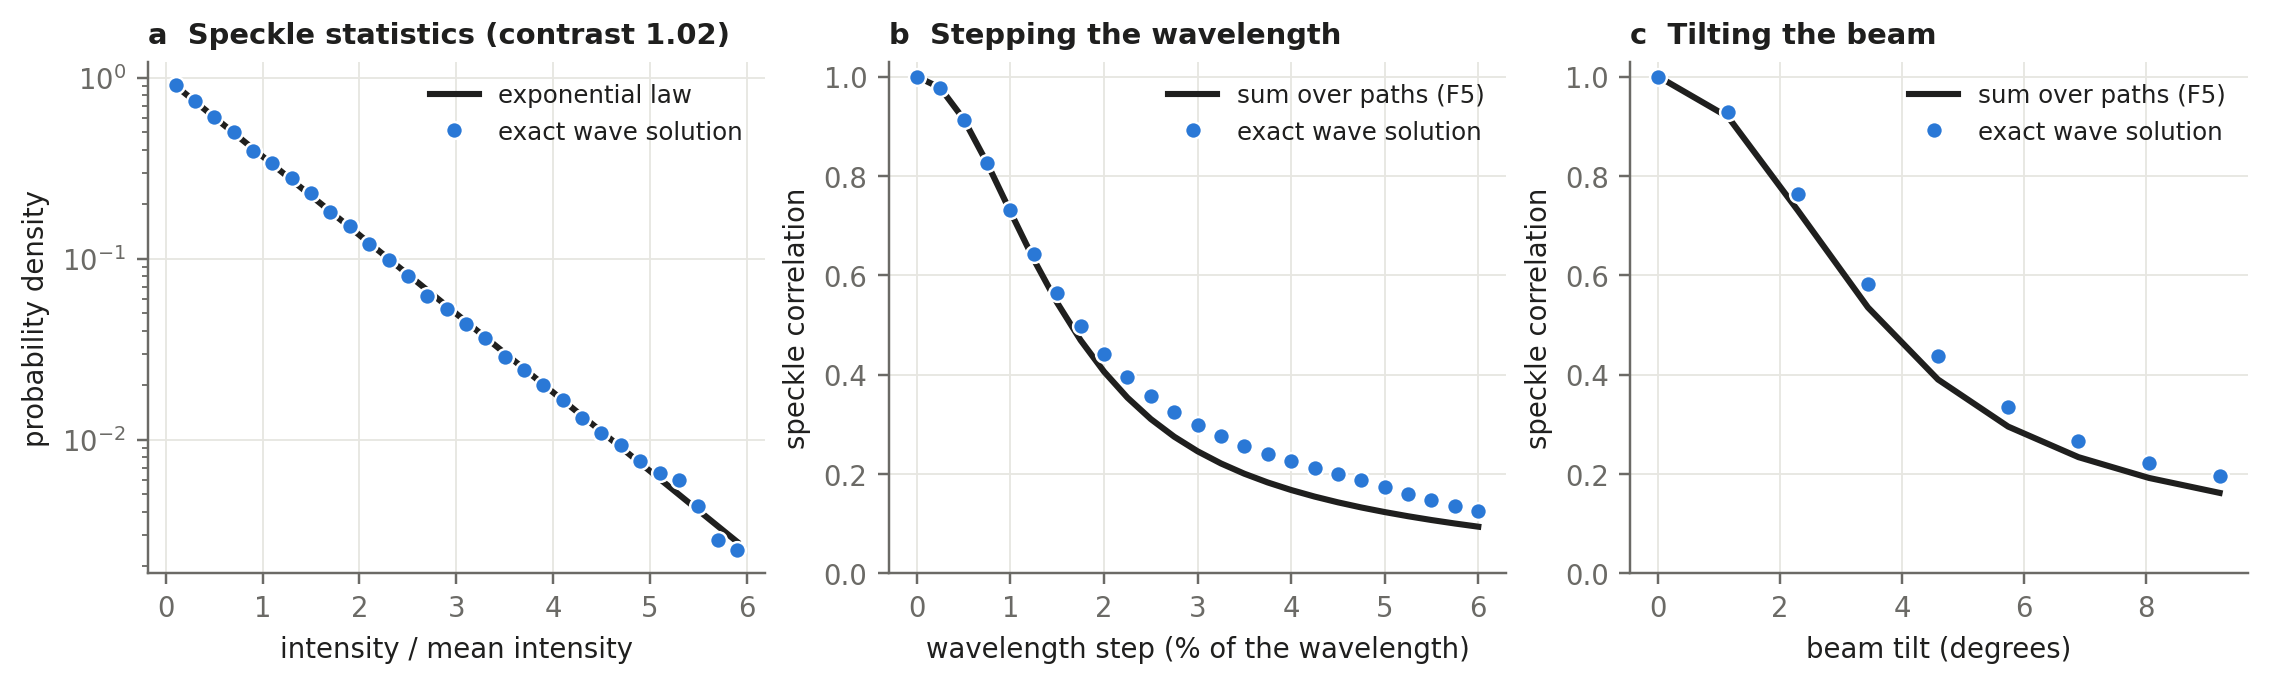
\includegraphics[width=\linewidth]{fig1_exact_wave.png}
\caption{Exact solution of the wave equation (markers) against the path formulas (lines), nothing fitted. (a) The
intensity follows the exponential law of fully developed speckle. (b) Speckle correlation when the wavelength is
stepped. (c) Speckle correlation when the beam is tilted, read at the correspondingly shifted direction.}
\end{figure}
The speckle contrast is \fwContrast{} (1 expected). The correlation curves differ from the path formula by at most
\fwSpecDiff{} (wavelength) and \fwTiltDiff{} (tilt); the prediction allowed 0.10. The exact solution decorrelates
slightly more slowly in the tails, which is expected for a sample where the mean free path is only 1.6 wavelengths.
So the two Fourier-transform statements (F3 and the tilt form of F4) hold in a solution of the wave equation itself.

\subsection*{Path lengths and polarization (Monte Carlo against diffusion)}
\begin{figure}[h!]
\centering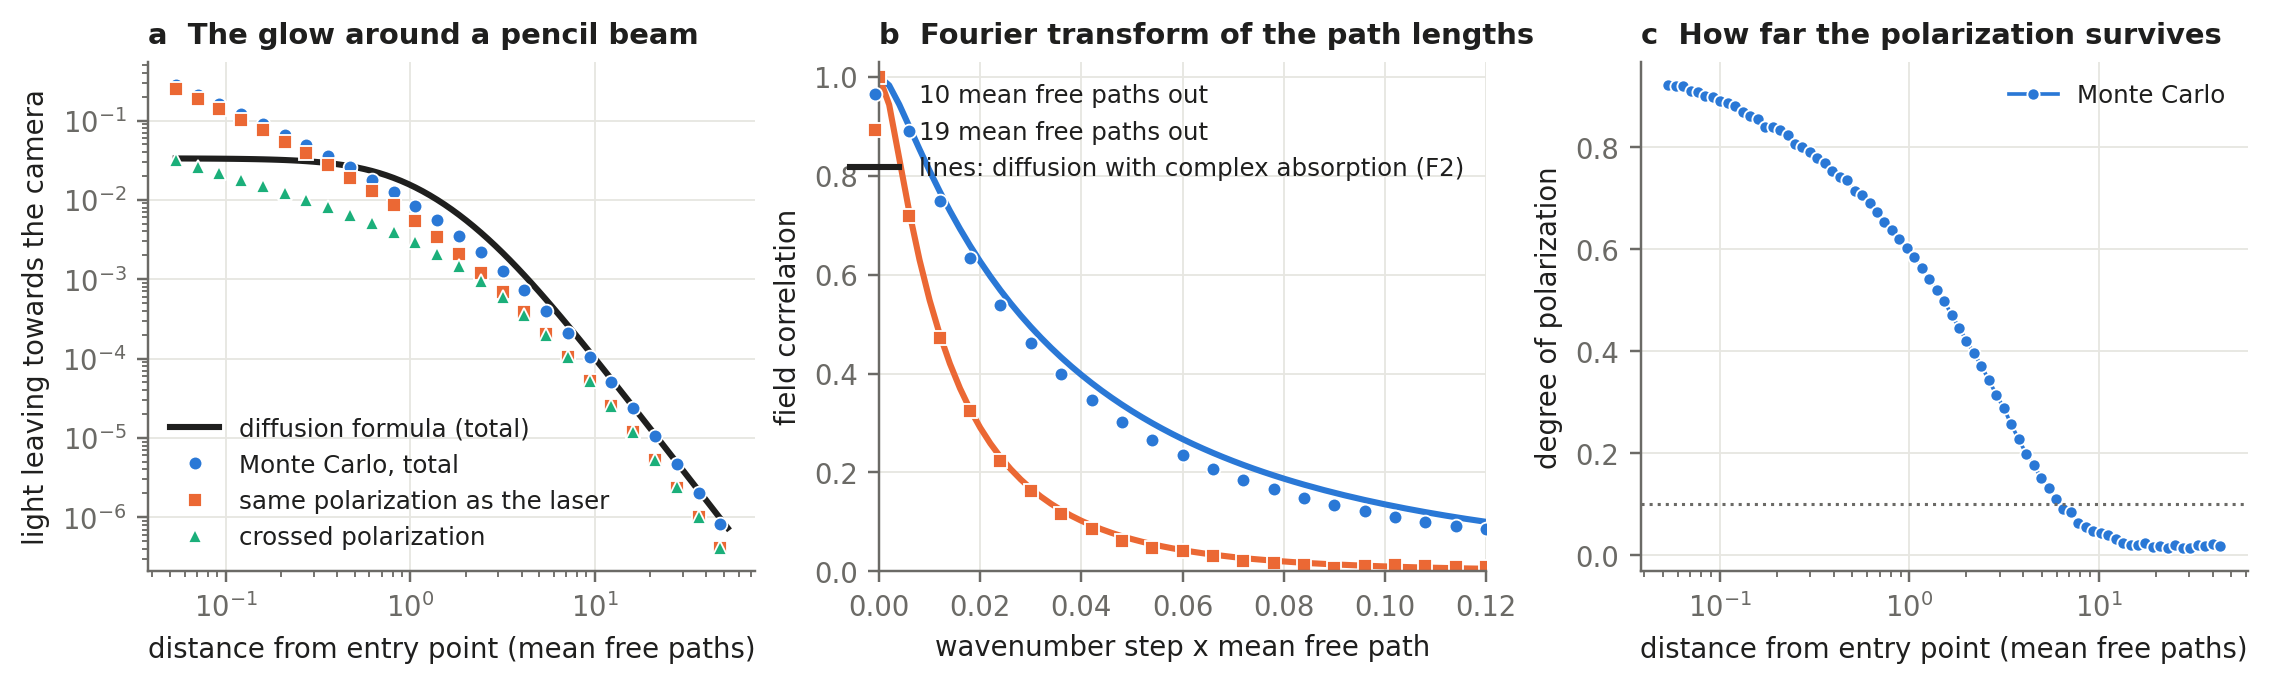
\includegraphics[width=\linewidth]{fig2_transport.png}
\caption{Path Monte Carlo. (a) Light leaving towards the camera around a pencil beam, split by polarization; the
diffusion formula holds beyond about 10 mean free paths. (b) The Fourier transform of the path lengths: Monte Carlo
(markers) against F2 (lines). (c) Degree of polarization against distance from the entry point.}
\end{figure}
F2 predicts the wavenumber step at which the field correlation halves within \dfTen\% at 10 mean free paths and
\dfTwenty\% at 19 (the prediction allowed 15\%). Close to the entry point diffusion fails, as it is known to, and the Monte Carlo is used there.
The light is depolarized (below 0.1) beyond \polDist{} mean free paths. I had predicted 5; at 5 it is still
\polAtFive.

\subsection*{Method 1: speckle degrees of freedom, ring by ring}
\begin{figure}[h!]
\centering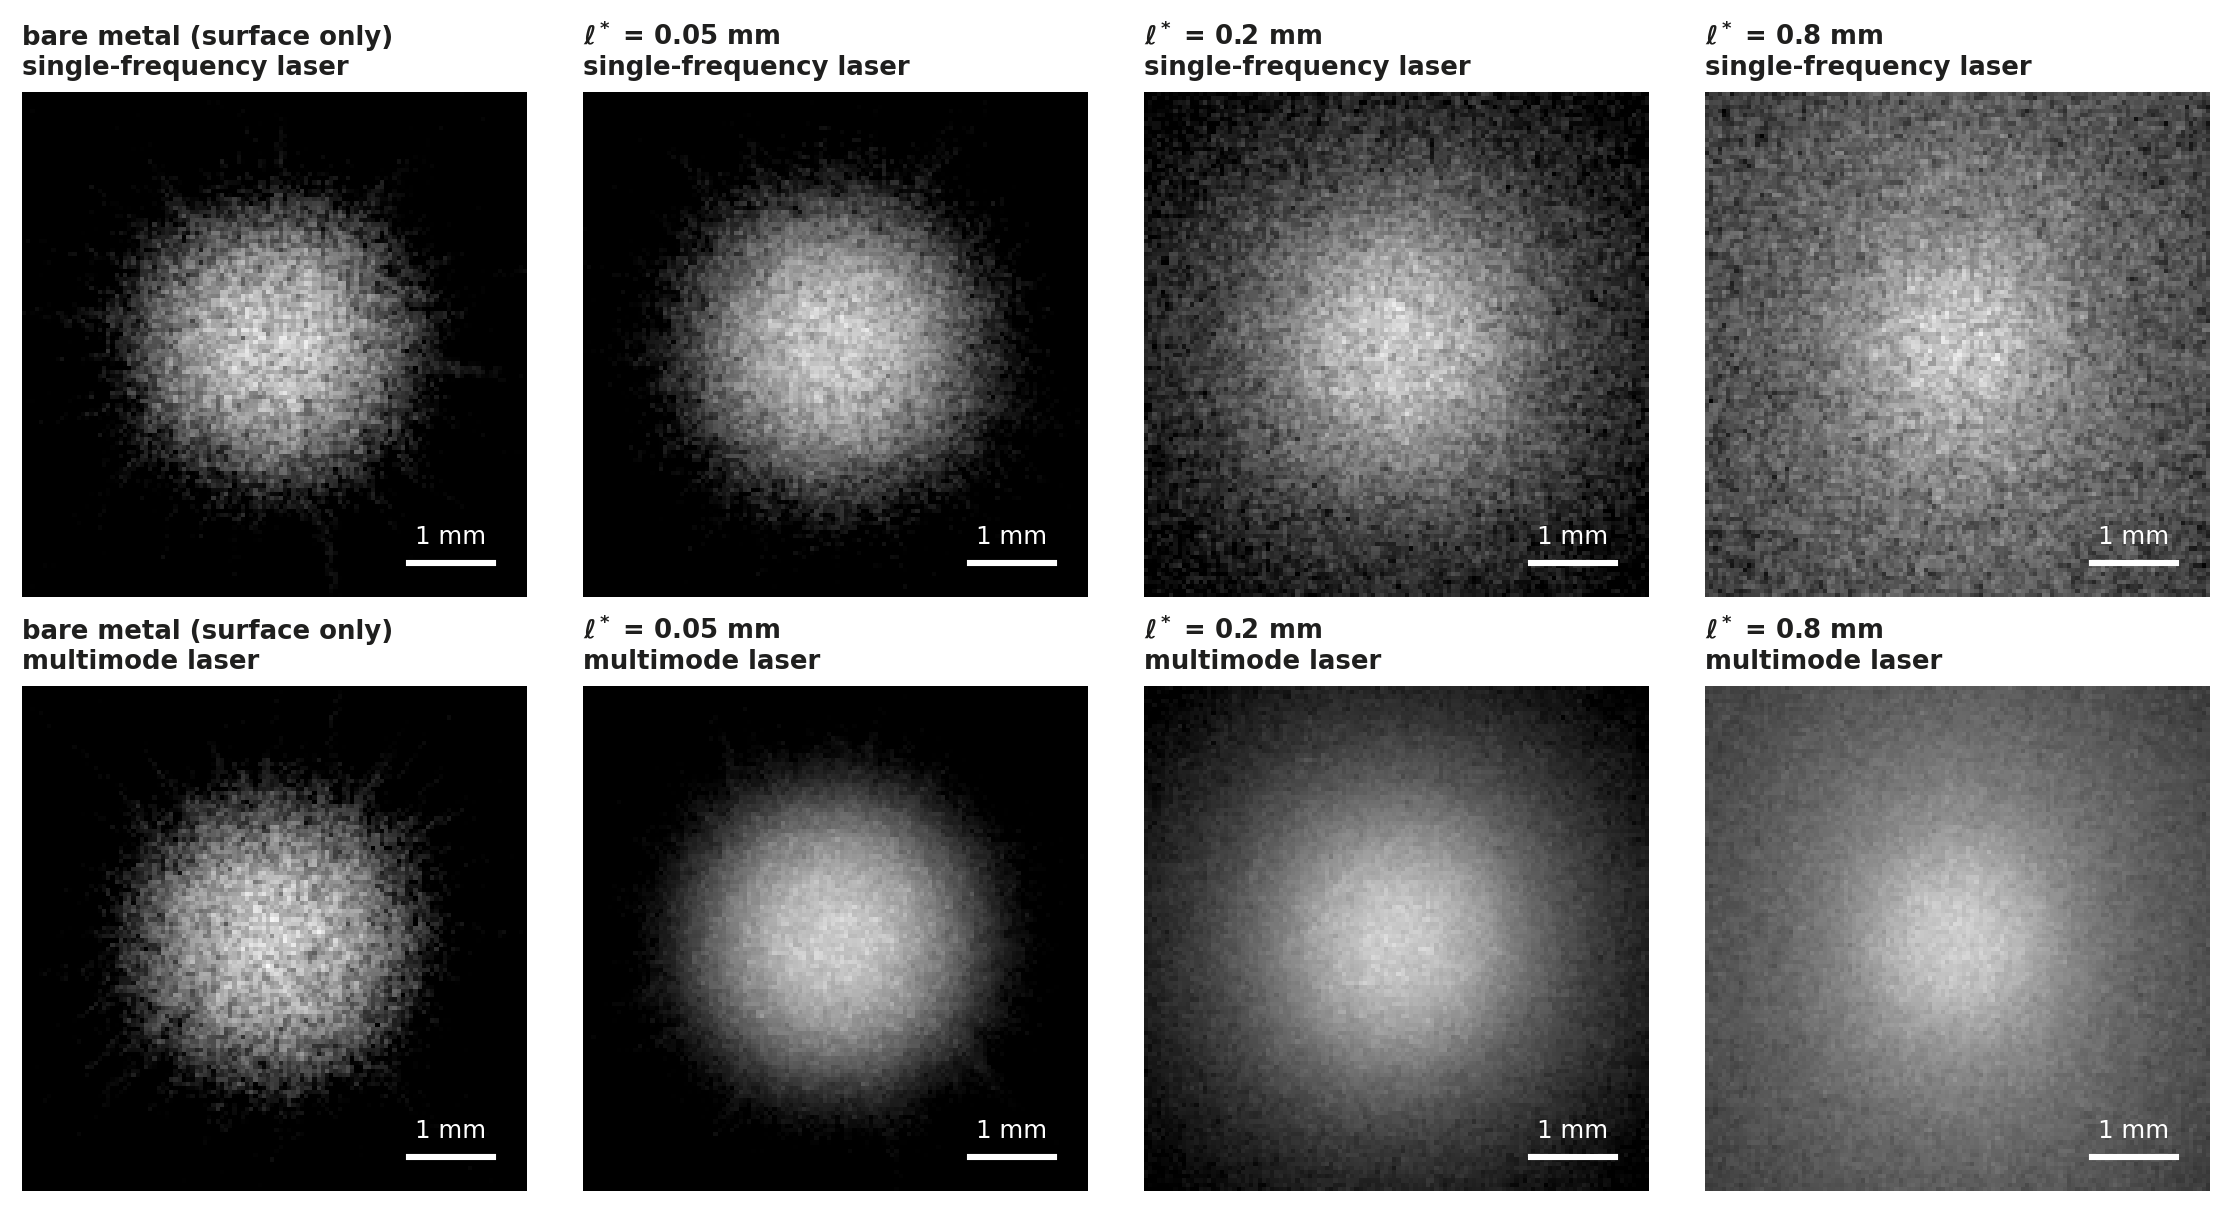
\includegraphics[width=\linewidth]{fig3_frames.png}
\caption{Simulated frames (logarithmic brightness, each normalized to its own centre). Top: single-frequency laser.
Bottom: multimode diode. On bare metal the speckle stays sharp. On the volume scatterers it washes out, more with the
multimode laser and more away from the centre.}
\end{figure}
\begin{figure}[h!]
\centering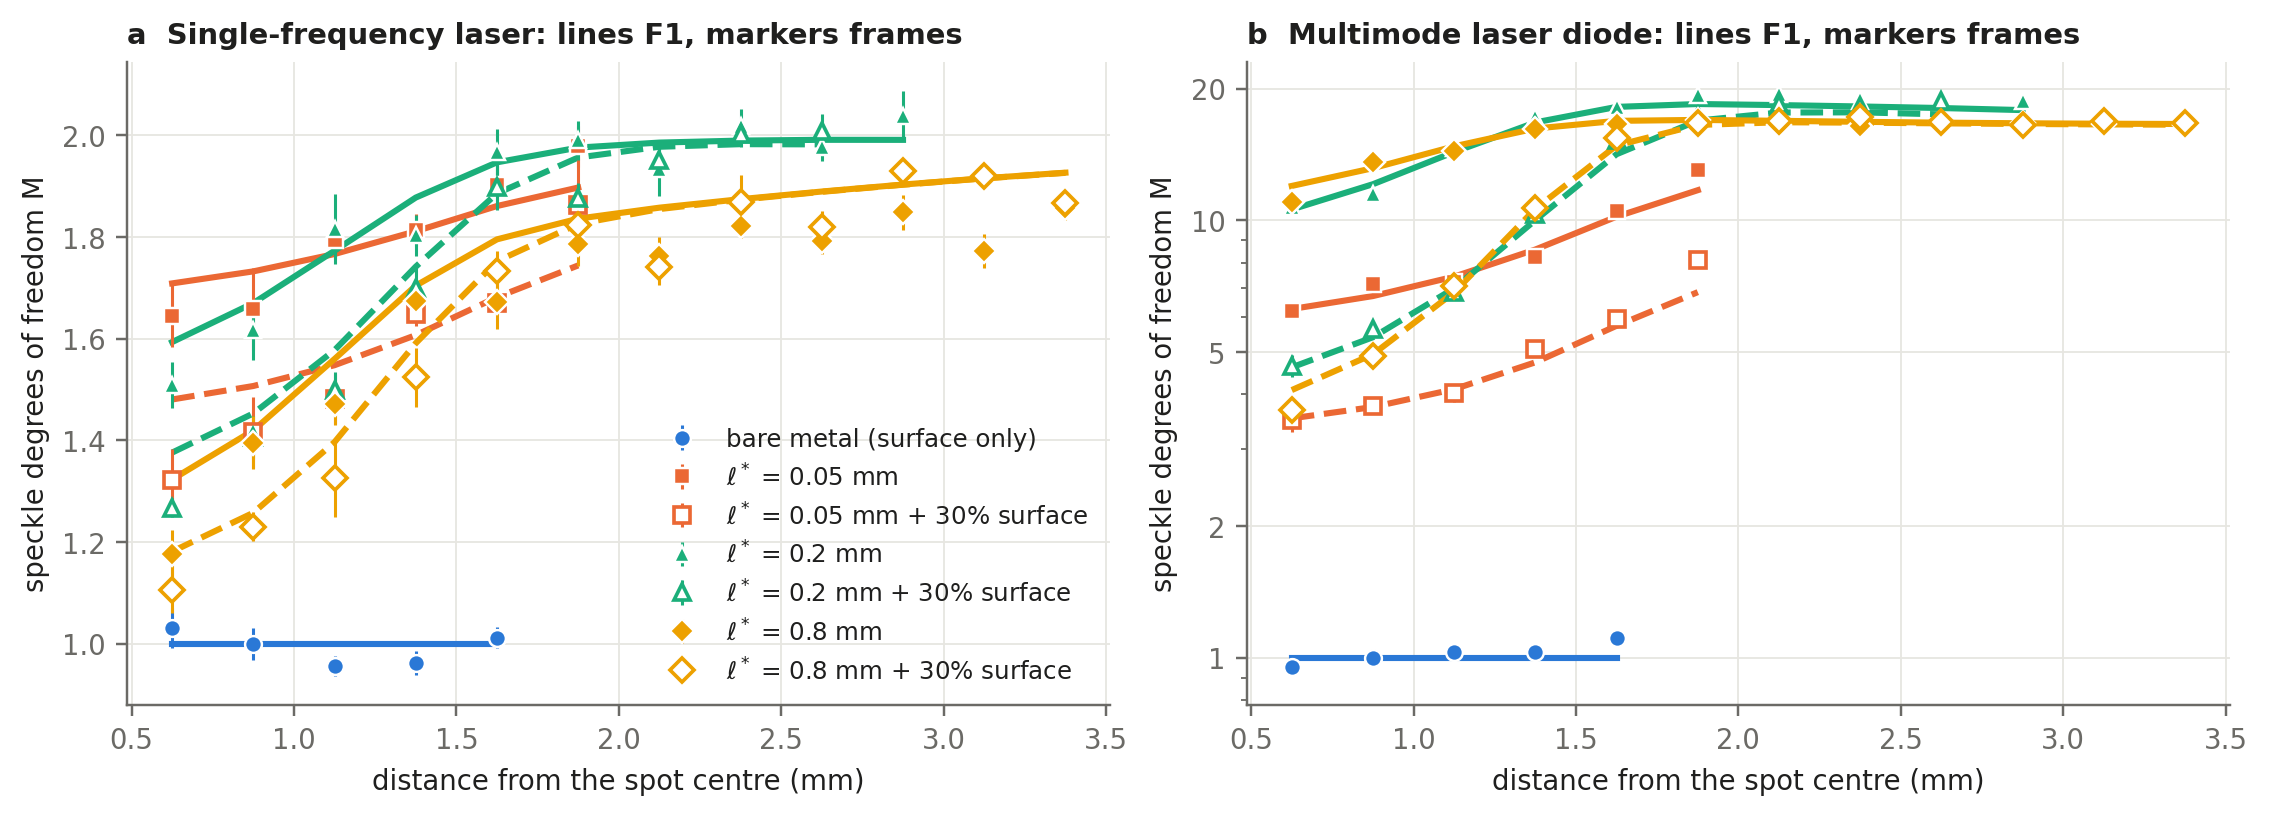
\includegraphics[width=\linewidth]{fig4_m_profiles.png}
\caption{$M$ against distance from the spot centre: formula F1 (lines) and the value measured from the simulated
frames (markers, \mObjects{} objects each, bars: standard error). Dashed and hollow: the same material with 30\%
surface light.}
\end{figure}
\mTable

\noindent The frames follow F1: the largest deviation over all scored rings is \mWorstSingle\% (single-frequency) and
\mWorstMulti\% (multimode). The prediction allowed 15\%, so the multimode case misses it by one point. That ring is
the dimmest one scored, where light from the bright core, diffracted by the lens, adds finer speckle; every other
ring is within 11\%. Reading of the figure:
\begin{itemize}
\item With a single-frequency laser $M$ only moves between 1 and 2. It separates surface light from light from
  inside, and little else.
\item With the multimode diode $M$ reaches \mMaxMulti{} and depends on both the transport length and the surface
  share, at the spot centre already. The short coherence length is what makes $M$ a path-length meter. $M$ levels off
  near twice the number of laser lines (about 10 here), once the paths differ by more than the distance over which
  the diode's coherence repeats, so the laser's spectrum sets the range of path lengths that $M$ can read.
\item The profile rises outward where the surface share falls; 30\% surface light pulls the centre down to
  $M\approx\mCoreSurf$ while the glow stays the same.
\item Far from the spot the lens's own diffraction of the bright core takes over (a real camera adds stray light
  there too), so the usable range ends where the glow drops to about $10^{-3}$ of the centre.
\end{itemize}

\subsection*{Method 1C: stepping the wavelength}
\begin{figure}[h!]
\centering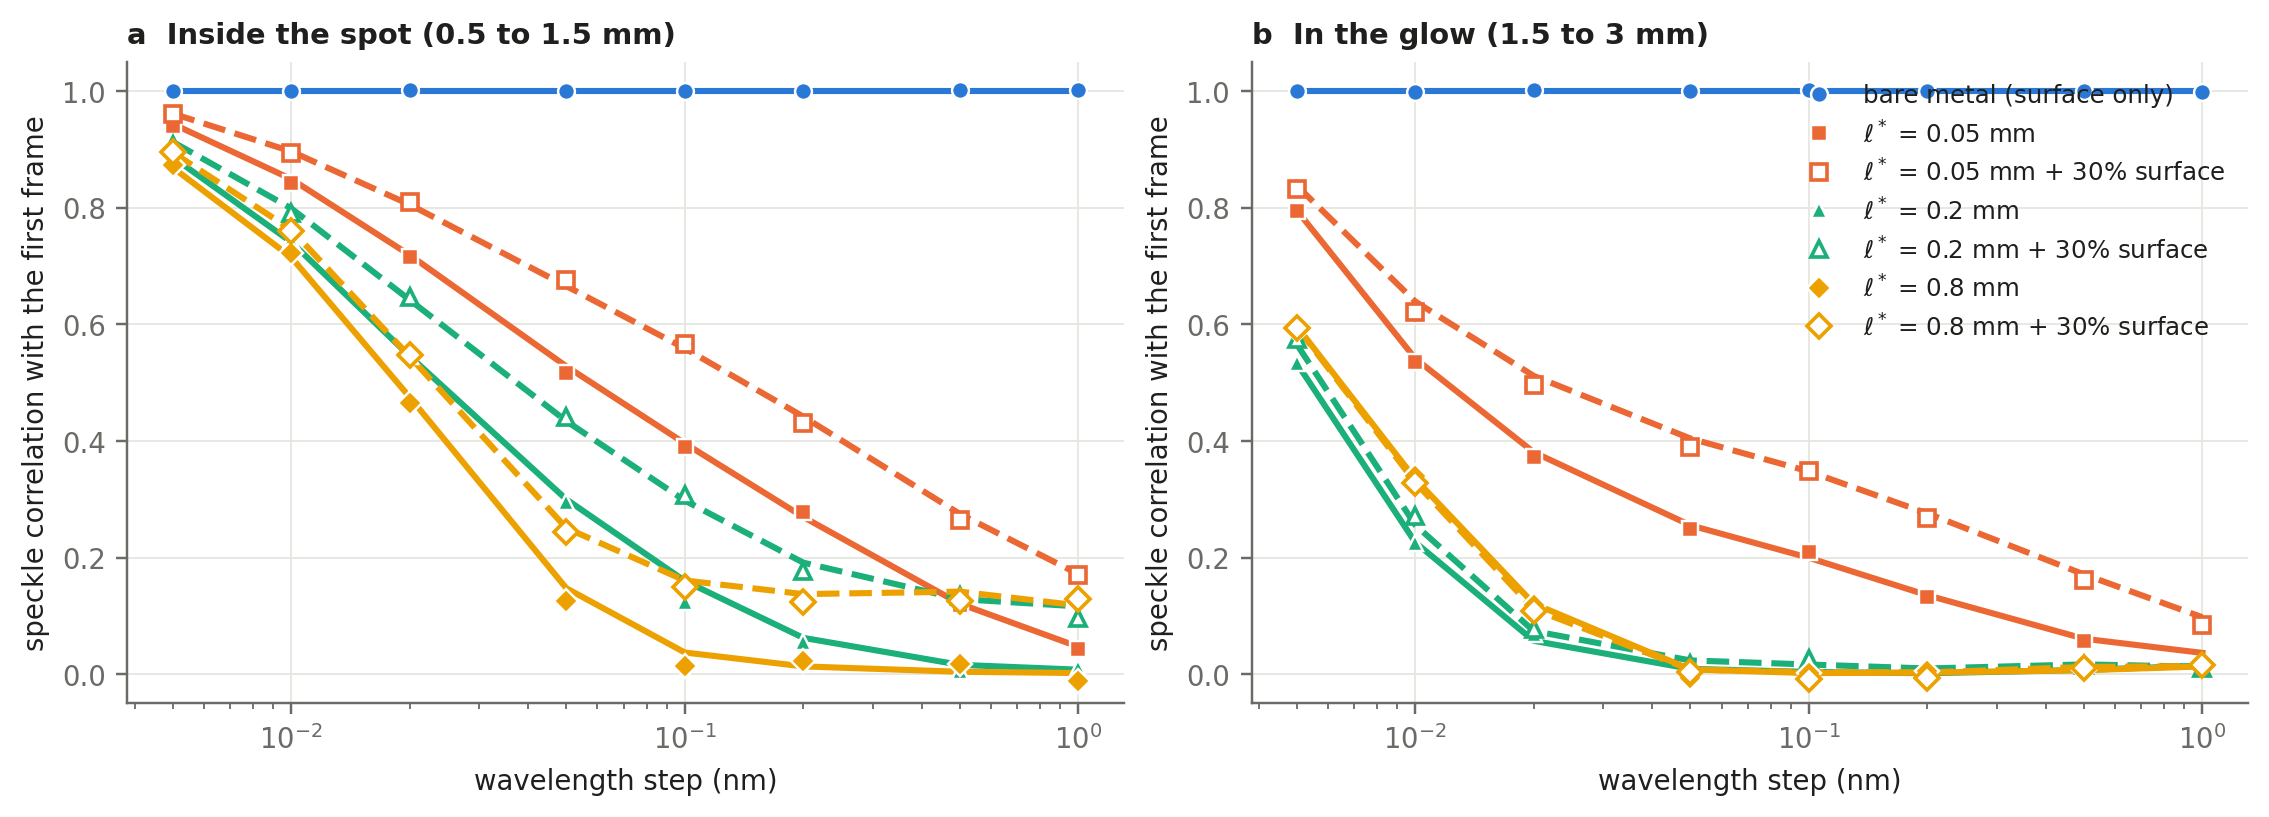
\includegraphics[width=\linewidth]{fig5_wavelength_steps.png}
\caption{Speckle correlation between a frame and frames taken at a stepped wavelength (single-frequency laser): F3
(lines) and simulated frames (markers).}
\end{figure}
\noindent Over all \wlCount{} ring-and-step values the frames differ from F3 by \wlRms{} on average (rms), with no
bias (\wlBias); the largest difference is \wlWorst{}, in the smallest ring. I had predicted 0.05 or less everywhere, and
\wlOver{} values exceed it, so that prediction is missed by sampling noise (\wlObjects{} objects per material). Metal
never decorrelates. The volume scatterers lose half their correlation at steps of \wlHalf: the longer the transport
length, the longer the paths inside the spot and the smaller the step. With 30\% surface light the curve levels off at
a plateau instead of going to zero. The steps needed are hundredths of a nanometre, which a temperature-tuned
single-frequency diode can do.

\subsection*{Method 4B: moving the beam}\label{sec:beam}
\begin{figure}[h!]
\centering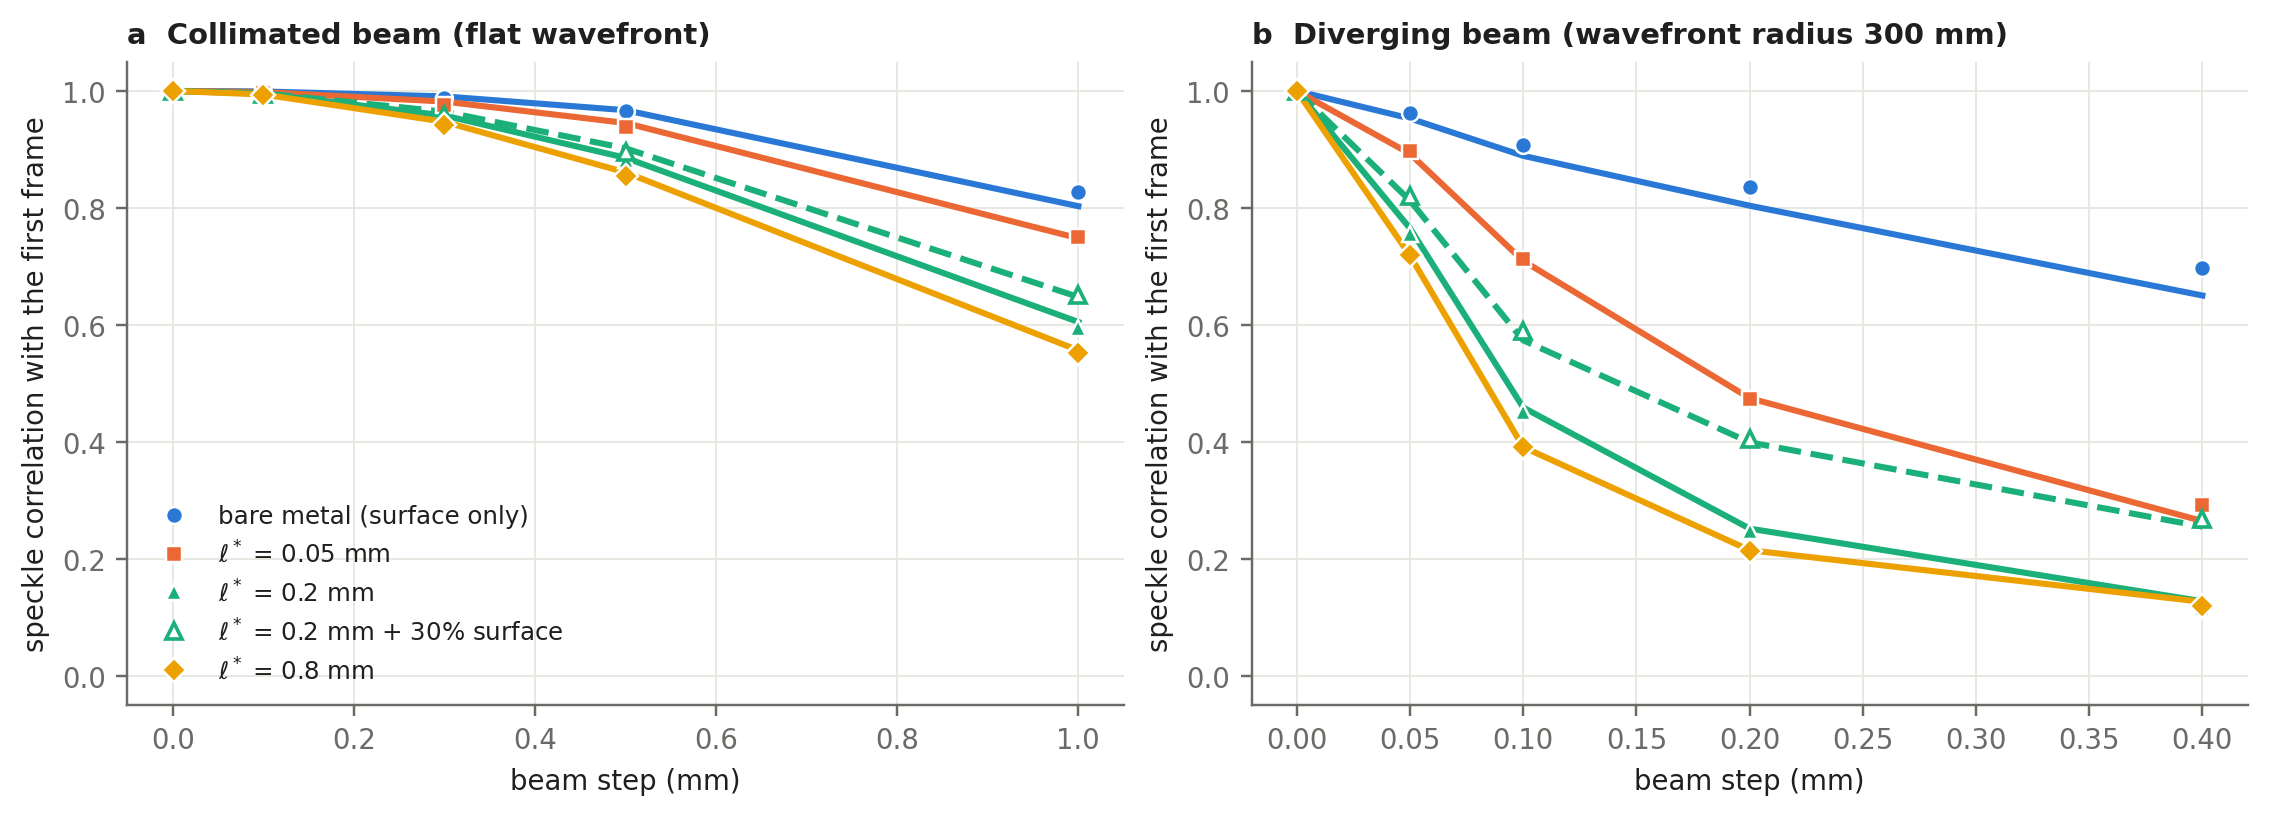
\includegraphics[width=\linewidth]{fig6_beam_steps.png}
\caption{Speckle correlation between a frame and frames taken after moving the beam (rings inside 1.5~mm): F4 (lines)
and simulated frames (markers). (a) Collimated beam. (b) The same beam with a wavefront radius of 300~mm.}
\end{figure}
\beamTable

\noindent Over all \beamCount{} ring-and-step values the frames differ from F4 by \beamRms{} on average (rms), bias
\beamBias, largest difference \beamWorst{} (\beamOver{} values above the predicted 0.05).
\begin{itemize}
\item \textbf{Collimated beam.} For steps up to $0.3\,w$ the surface-only and volume-only correlations differ by at
  most \beamFlatGap{} (the lowest value in any ring is \beamFlatMin). The test as I described it on 20 November (``move the beam a fraction of a millimetre: surface
  speckle stays, speckle from inside changes'') does not work with a collimated beam. Only at a step equal to the
  beam radius do the materials separate (\beamFlatAtW).
\item \textbf{Diverging beam, $R_c=300$~mm.} At a step of \beamBestStep~mm the metal is still at \beamBestMetal{}
  while the volume scatterers are at \beamBestVol. The step that halves the correlation measures the sideways travel
  of light inside the material (rms \beamSpread~mm for the three materials). I had predicted a step with surface
  light above 0.9 and volume light below 0.5; at 0.1~mm they are \beamTenthMetal{} and \beamTenthVol, so that wording is
  missed by 0.01.
\item The strong scatterer ($\ell^*=0.05$~mm) spreads light by about what the lens resolves here (0.15~mm), so it
  falls between the metal and the other two. More zoom moves that limit.
\item Towards the edge of the spot the metal falls faster than at the centre, because the lens's diffraction carries
  in light from the bright core. For bare metal the frames sit \beamMetalBias{} above the formula on average: pixels
  average the cross term a little less than the formula's point value assumes (on unbinned frames the difference
  disappears).
\end{itemize}

\section{What this means for the rig}\label{sec:rig}
\begin{itemize}
\item \textbf{Zoom in (your note that the focal length is adjustable).} Ring statistics need many grains per ring.
  A ring of radius $r$ and width $\Delta r$ holds about $2\pi r\,\Delta r/A_c$ grains, with $A_c\approx0.21\,g^2$ for
  a grain of diameter $g$, and the relative error of $M$ is between $\sqrt{2/N}$ and $\sqrt{8/N}$ for $N$ grains.
  With grains of 3~pixels the beam should be at least 40~pixels across; the simulation used that. In the 800-pixel
  scanner previews the spot is only a few pixels wide and a grain is smaller than a pixel, which is why nothing could
  be read there. Bigger is better, as you said.
\item \textbf{Aperture.} A grain on the sensor is about $2.4\,\lambda\times$ f-number (12~\textmu m at f/8 and
  635~nm). It has to cover 2 pixels or more, so the lens must be stopped down. Zoom sets how many grains the spot
  covers; the f-number sets how many pixels a grain covers.
\item \textbf{Exposure.} No clipped pixels: three bracketed exposures per laser, merged. Two frames per laser, and
  one with the lasers off. Uncompressed files, sharpening and denoising off.
\item \textbf{Laser.} For method 1 a cheap multimode diode is the better choice. Its coherence function has to be
  measured once on bare metal and on one known diffuser, like the beam width. For wavelength steps (1C) one
  temperature-tuned single-frequency diode is needed.
\item \textbf{Beam steps on the arm.} Focus the laser module so the beam diverges from a point about 300~mm in front
  of the object, then step 0.05 to 0.2~mm. The camera must not move with the beam. A collimated beam needs steps of
  about the beam radius instead.
\item \textbf{Projector.} Noted that it is unplugged so the lasers stand out. I will plug it back in only for the
  fringe captures (method 2C).
\end{itemize}

\section{Limits}
\begin{itemize}
\item This tests the math and the estimators. It says nothing yet about accuracy on real objects.
\item The materials are parameter sets, not measured samples. The scatterers are small (Rayleigh); real materials
  have larger particles and fibres, which change the numbers (not the formulas, which hold for any kernel $K$ and any
  $W$).
\item Polarization is simulated for a surface without internal reflection. A second kernel with $n=1.4$ was computed
  but not yet used.
\item The lens is ideal and the laser spectrum is assumed.
\item The exact wave solution is scalar and small; it checks the path picture, not polarization.
\end{itemize}

\section{Next}\label{sec:next}
\begin{enumerate}
\item \textbf{Synthetic training data} (your suggestion). The frame generator can draw any number of objects with
  random transport length, absorption, surface share, brightness and surface print. Train the readout on them and test
  whether it ignores brightness and print.
\item \textbf{Pilot capture} on 10 to 12 objects with the settings of Section~\ref{sec:rig}: zoomed in, stopped down,
  three exposures, two frames per laser. Fit $\ell^*$ and the surface share from $M(r)$ and the brightness profile,
  and run checks (a) to (d).
\item \textbf{Measure our lasers' coherence} (bare metal plus one diffuser), since $M$ depends on it.
\item \textbf{Extend the simulator}: larger particles, internal reflection, fibres (wood, paper, fabric).
\end{enumerate}

\end{document}
